%%%%%%%%%%%%%%%%%%%%%%%%%%%%%%%%%%%%%%%%%%%%%%%%%%%
%																													
%																												
%																													
%									Importations	de bibliothèques	
%																													
%																												
%%%%%%%%%%%%%%%%%%%%%%%%%%%%%%%%%%%%%%%%%%%%%%%%%%%


\documentclass[hidelinks]{article}
\usepackage[utf8]{inputenc}
\usepackage{graphicx}
\usepackage[T1]{fontenc}
\usepackage[french]{babel}
\usepackage{csquotes}
\usepackage[section]{placeins}
\usepackage{tikz}
\usepackage{hyperref}
\usepackage{afterpage}
\usepackage{pdfpages}
\usepackage{wrapfig}
\usepackage{amsmath, mathtools}
\usepackage{amssymb}
\usepackage{fancyhdr}
\usepackage[all]{background}
\usepackage{appendix}


%%%%%%%%%%%%%%%%%%%%%%%%%%%%%%%%%%%%%%%%%%%%%%%%%%%%%%%%%%%%%%%%%%%%
%																																	   %
%																																	   %
%																																	   %
%															Page de garde															   %
%																																	   %
%																																	   %
%%%%%%%%%%%%%%%%%%%%%%%%%%%%%%%%%%%%%%%%%%%%%%%%%%%%%%%%%%%%%%%%%%%%



\newcommand{\MyGraphicLogo}{% For imported graphic logo
\begin{tikzpicture}[remember picture,overlay,yshift=-15cm, xshift=10.5cm]
	\definecolor{gris}{RGB}{16,52,78}
	\definecolor{jaune_fonce}{RGB}{0, 107, 163}
	\definecolor{jaune}{RGB}{0, 151, 136}
	\fill [gris] (-10.5,-10) -- (0,-4.5) -- (14,-13) -- (14,-16)--(0,-16)--(-10.5,-16);
	\fill [jaune_fonce] (0,-4.5) -- (-10.5,-10) -- (-10.5, 1.8);
	\node at (3.8,0.4) {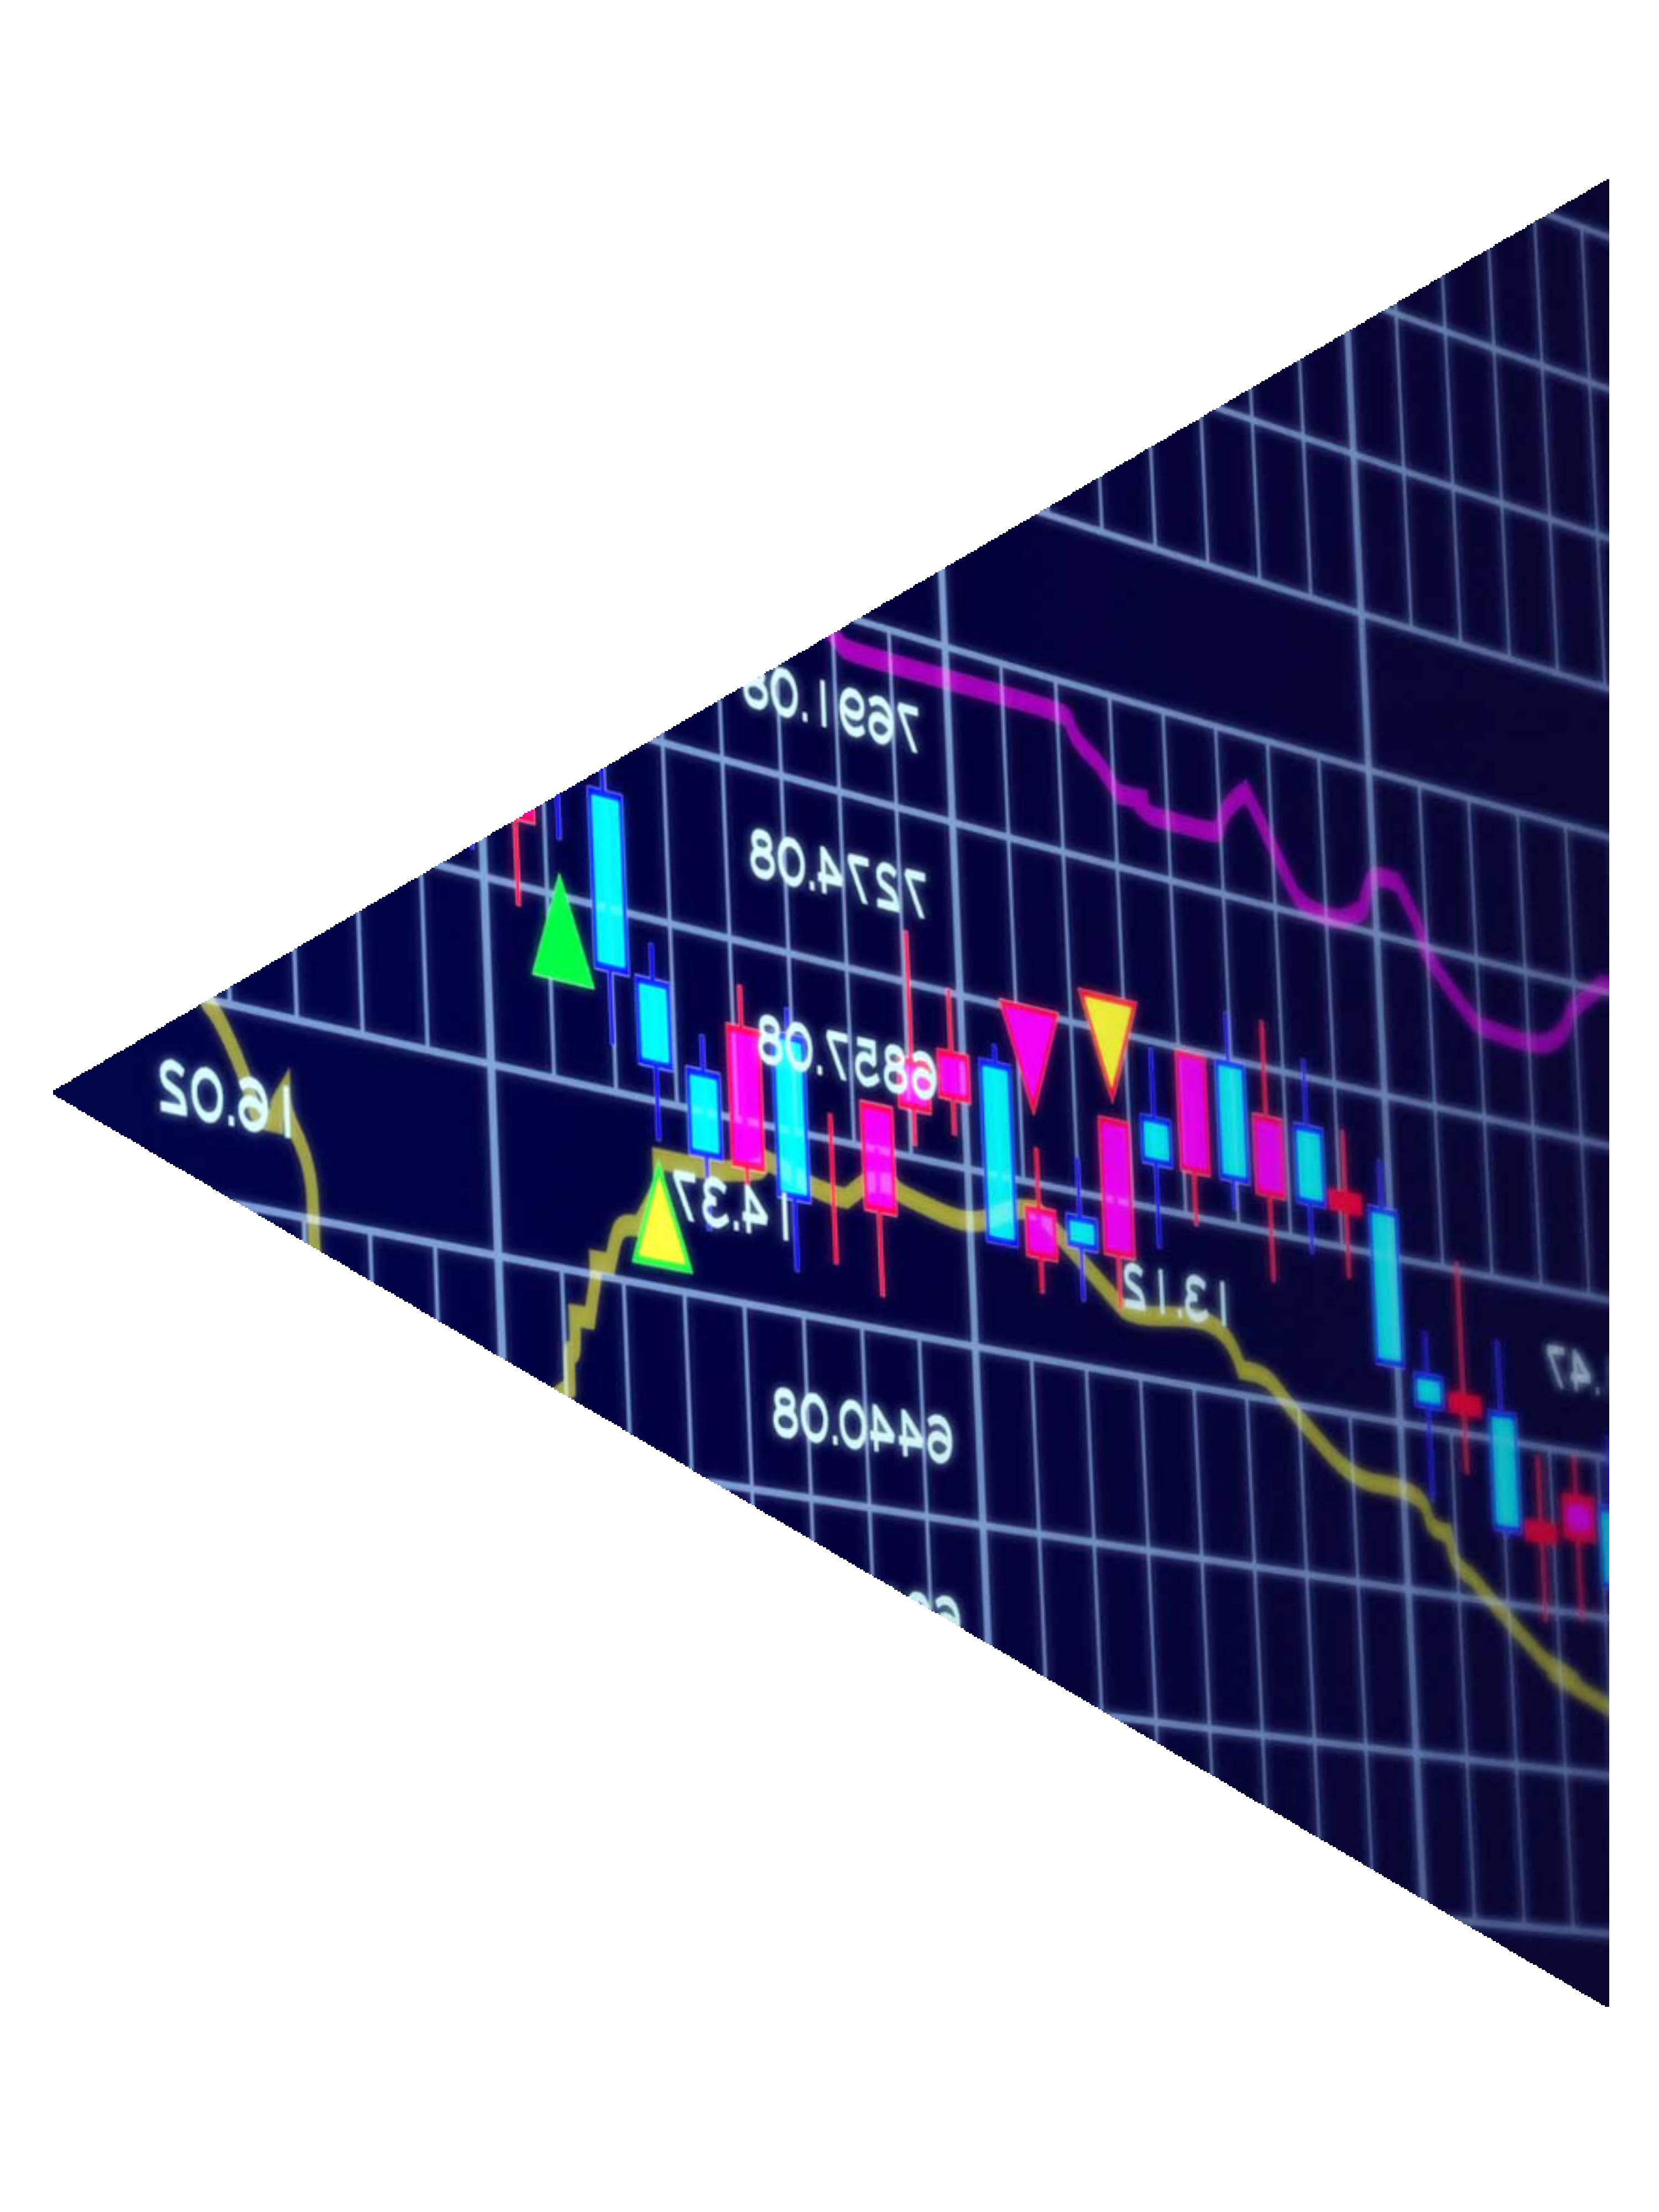
\includegraphics[width=22cm]{triangle.png}};
	\fill [jaune] (14,5) -- (2.5, 12) -- (20,25) -- (14, 20);
 \end{tikzpicture}}


\SetBgContents{\MyGraphicLogo}% Select included image

\SetBgPosition{current page.north west}% Select location
\SetBgOpacity{1.0}% Select opacity
\SetBgAngle{0.0}% Select roation of logo
\SetBgScale{1.0}% Select scale factor of logo



%%%%%%%%%%%%%%%%%%%%%%%%%%%%%%%%%%%%%%%%%%%%%%%%%%%%%%%%%%%%%%%%%%%%
%																																	   %
%																																	   %
%																																	   %
%										Informations générales sur le document															   %
%																																	   %
%																																	   %
%%%%%%%%%%%%%%%%%%%%%%%%%%%%%%%%%%%%%%%%%%%%%%%%%%%%%%%%%%%%%%%%%%%%

 \usepackage{fontspec}
  \usepackage[bold-style=upright]{unicode-math}
  \defaultfontfeatures{Scale=1}
  \setmainfont[Ligatures=TeX,Numbers=OldStyle]{Lucida Bright OT}
  \setmathfont[RawFeature=+ss04]{Lucida Bright Math OT}
  \setsansfont[Scale=1.0,Numbers=OldStyle]{Myriad Pro}
  \newfontfamily\fullcaps[Letters=Uppercase,Numbers=Uppercase]{Myriad Pro}
  \usepackage[babel=true]{microtype}
  \usepackage{icomma}
  
  
  
  
  
  
  
  
  
  
  
\title{Variance reduction methods}
\author{Maxence COUPET - \href{mailto:maxence.coupet@gmail.com}{maxence.coupet@gmail.com}}
\date{March 2018}



\MHInternalSyntaxOn
\MH_set_boolean_T:n {outer_mult}
\MHInternalSyntaxOff

\newenvironment{nalign}{
    \begin{equation}
    \begin{aligned}
}{
    \end{aligned}
    \end{equation}
    \ignorespacesafterend
}

\usepackage{listings}
\usepackage{color}

\definecolor{mygreen}{rgb}{0,0.6,0}
\definecolor{mygray}{rgb}{0.5,0.5,0.5}
\definecolor{mymauve}{rgb}{0.58,0,0.82}

\lstset{ 
  backgroundcolor=\color{white},   % choose the background color; you must add \usepackage{color} or \usepackage{xcolor}; should come as last argument
  basicstyle=\footnotesize,        % the size of the fonts that are used for the code
  breakatwhitespace=false,         % sets if automatic breaks should only happen at whitespace
  breaklines=true,                 % sets automatic line breaking
  captionpos=b,                    % sets the caption-position to bottom
  commentstyle=\color{mygreen},    % comment style
  deletekeywords={...},            % if you want to delete keywords from the given language
  escapeinside={\%*}{*)},          % if you want to add LaTeX within your code
  extendedchars=true,              % lets you use non-ASCII characters; for 8-bits encodings only, does not work with UTF-8
  frame=single,	                   % adds a frame around the code
  keepspaces=true,                 % keeps spaces in text, useful for keeping indentation of code (possibly needs columns=flexible)
  keywordstyle=\color{blue},       % keyword style
  language=Octave,                 % the language of the code
  morekeywords={*,...},            % if you want to add more keywords to the set
  numbers=left,                    % where to put the line-numbers; possible values are (none, left, right)
  numbersep=5pt,                   % how far the line-numbers are from the code
  numberstyle=\tiny\color{mygray}, % the style that is used for the line-numbers
  rulecolor=\color{black},         % if not set, the frame-color may be changed on line-breaks within not-black text (e.g. comments (green here))
  showspaces=false,                % show spaces everywhere adding particular underscores; it overrides 'showstringspaces'
  showstringspaces=false,          % underline spaces within strings only
  showtabs=false,                  % show tabs within strings adding particular underscores
  stepnumber=2,                    % the step between two line-numbers. If it's 1, each line will be numbered
  stringstyle=\color{mymauve},     % string literal style
  tabsize=2,	                   % sets default tabsize to 2 spaces
  title=\lstname                   % show the filename of files included with \lstinputlisting; also try caption instead of title
}

 
%%%%%%%%%%%%%%%%%%%%%%%%%%%%%%%%%%%%%%%%%%%%%%%%%%%%%%%%%%%%%%%%%%%%
%																																	   %
%																																	   %
%																																	   %
%												Mis en page du document																   %
%																																	   %
%																																	   %
%%%%%%%%%%%%%%%%%%%%%%%%%%%%%%%%%%%%%%%%%%%%%%%%%%%%%%%%%%%%%%%%%%%%


\begin{document}
	\selectlanguage{french}
	% page de garde
	\pagenumbering{gobble}
	\maketitle
	\newpage
	% début du rapport
	
	
	


\newcommand{\MyGraphicLog}{% For imported graphic logo
\begin{tikzpicture}[remember picture,overlay,yshift=-15cm, xshift=10.5cm]
\definecolor{jaune}{RGB}{16, 52, 78};
\fill[jaune] (-11, -16) -- (13, -16) -- (13, -12.1) -- (-11, -12.1);
 \end{tikzpicture}}


\SetBgContents{\MyGraphicLog}% Select included image


\SetBgPosition{current page.north west}% Select location
\SetBgOpacity{1.0}% Select opacity
\SetBgAngle{0.0}% Select roation of logo
\SetBgScale{1.0}% Select scale factor of logo

\pagestyle{fancy}
\renewcommand\headrulewidth{0pt}
\lhead{}\chead{}\rhead{}
\cfoot{\vspace*{6\baselineskip} \textcolor{white}{\thepage} \large}
	\newpage

	\pagenumbering{arabic}

%%%%%%%%%%%%%%%%%%%%%%%%%%%%%%%%%%%%%%%%%%%%%%%%%%%%%%%%%%%%%%%%%%%%
%																																	   %
%																																	   %
%																																	   %
%								Début du document (commencez à taper votre texte ici)													   %
%																																	   %
%																																	   %
%%%%%%%%%%%%%%%%%%%%%%%%%%%%%%%%%%%%%%%%%%%%%%%%%%%%%%%%%%%%%%%%%%%%
When simulating stochastic processes in order to compute the price of a derivative, we have to compute a lot of paths in order to be accurate, which could be very time consumming. All the following methods allow one to make the simulated price converging faster to its limit.
	\section{Confidence bounds}
	
	Computing the price of a derivative using the Monte-Carlo method implies to generate $N$ different paths for the underlying, then computing the payoff for each of these paths, computing the mean of all payoffs and finally discounting the value in order to get the present value of the derivative. 
	
	According to the central limit theorem, we have the following confidence bounds at a $95\%$ level :
	$$\hat{\mu}-\frac{1.96\hat{\sigma}}{\sqrt{N}}<derivative\quad price<\hat{\mu}+\frac{1.96\hat{\sigma}}{\sqrt{N}}$$
	with $\hat{\mu}$ the empirical mean and $\hat{\sigma}$ the empirical standard variation.
	
	With this formula we have only two options to improve the confidence bounds : increasing the number of simulations $N$ or reducing $\hat{\sigma}$. The following methods are meant to reduce the variance and while they are presented individually they are often applied together.
	
	We will test the method on a standard laptop within a single threaded program. While using multi threading is really usefull for reducing time of execution, it is used to increase the number of simulations and thus is not in the scope of this document which focuses on variance reduction.
	
	\newpage
	\section{Antithetic variates}
	The main idea with this method is to compute two values of the derivative price at each simulation. The first value will be computed as usual with the random path, but another will be computed with the opposite path. For example if for the path $n$ the value at the time $t$ for the underlying is : $S_n (t)=S_n(0)e^{(r-\frac{\sigma^2}{2})t+\sigma\epsilon}$, the value of the opposite path at the same time will be : $S_n^{'}(t)=S_n(0)e^{(r-\frac{\sigma^2}{2})t-\sigma\epsilon}$, where $\epsilon$ is a sample from a random variable following a standard normal law (see figure \ref{fig:opposite}).
	\begin{figure}[!h]
				\centering
				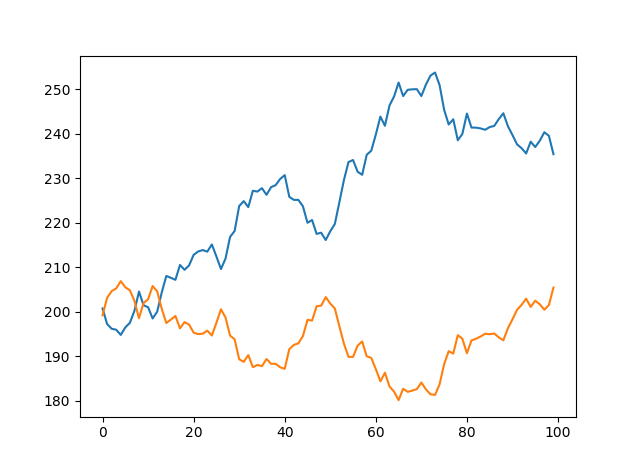
\includegraphics[width=0.8\linewidth]{opposite_path.png}
				\caption{Example of paths used for the antithetic variates method}
				\label{fig:opposite}
				\end{figure}
	
	It is very important to understand that we take opposite values for the standard normal random variable which represent the random part of the price, not the opposite values of prices themselves. Since the stochastic process representing the underlying has log normal returns, the two path will not be exactly symetric when we plot then together, as we can see on figure \ref{fig:opposite}.
	
	Since with the same number of simulations, we get twice as much price observations for the derivative, we need half of the initial number of simulations to get the same amount of observations. This is interesting because generating a (pseudo-)random number is a process that is time consuming in a computer program, and with this method we are generator half of the number generated normally, we then could expect the time of execution to be reduced.
	
	In order to empirically test this, we will use a Python script (see the \hyperref[sec:antithetic]{annexe} for source code). We will compute the price of an european call on a stock paying no dividend for several number of simulations, and will look very carefully to the difference of time of execution and the speed of convergence to the mean for a classical simulation and the antithetic variates method.
	
	\begin{figure}[!h]
				\centering
				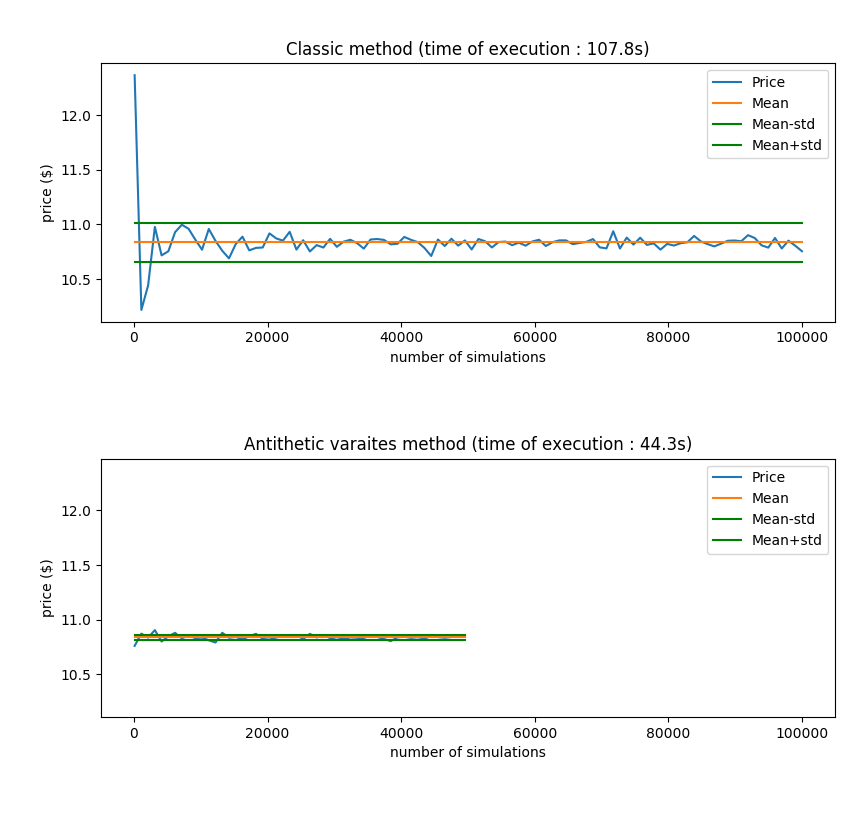
\includegraphics[width=\linewidth]{antithetic.png}
				\caption{Comparaison of the two methods}
				\label{fig:antithetic}
				\end{figure}
				
	As we can see on figure \ref{fig:antithetic}, the antithetic variates method is much faster to converge to the mean than the classic method (x and y axis are the same for both charts). Moreover execution time is half the one of classical method, therefore it is both faster to converge and faster in execution time. Nonetheless, we have to keep in mind that we are here dealing with vanilla option with a payoof very easy (and fast) to compute. For more exotic options, especially path-dependant options, the amount of execution time spent of computing the payoff  would be much more important and thus the net gain in execution time would not be that big, but it will not change anything to the relative speed of convergence to the mean value as long as the price is monotonic with respect to the underlying price. 
	
	In order to explain why this method converge much faster, we have to remender how to reduce the confidence interval : reduce the variance.
	
	Let's consider $S_1$ and $S_2$ two sample paths. We want an estimation of $\theta=\mathbb{E}(S)$, which is given by the unbiased estimator : $\hat{\theta}=\frac{\hat{\theta_1}+\hat{\theta_2}}{2}$. We then  have :
	$$Var(\hat{\theta})=\frac{Var(S_1)+Var(S_2)+2Cov(S_1,S_2)}{4}$$
	
	With the above formula, it is clear why we are taking opposite values for the random path : the minimal variance is obtained when both path are negatively correlated ($Cov(S_1,S_2)=-1$).
	
\newpage
\section{Control variates}
The key idea with the control variates method is that if a simulation misprice a derivative A with an error $\epsilon$, it will also misprice another related derivative B with the same error $\epsilon$. In order to use this method, we first compute the analytic price of the derivative A, then we compute with a simulation an approximation of the price of derivative A and we store the error. Finally we compute an approximation of the price of derivative B and then substract the error. We then have the following equality :
$$P_B=\hat{P}_B - \hat{P}_A + P_A$$
with $P_B$ the price we want to compute, $\hat{P}_B$ the price of derivative B obtained with a simulation, $\hat{P}_A$ the price of derivative A obtained with a simulation and $P_A$ the analytic price of derivative A.

A more general method will use a multiplicating factor for the error :
$$P_B=\hat{P}_B - k(\hat{P}_A - P_A), \quad k \in \mathbb{R}$$

Again, the goal is to reduce the variance. Here the variance of $P_B$ is given by :
$$Var(P_B)=Var(\hat{P}_B)+k^2 Var(\hat{P}_A) + 2kCov(\hat{P}_B,\hat{P}_A)$$

One can proove (by computing the partial derivative of the above equation with respect to $k$, and setting it equal to $0$) that the optimal value for $k$ is :
$$k_{opt} = -\frac{Cov(\hat{P}_B,\hat{P}_A)}{Var(\hat{P}_A)}$$

Unfortunately, gathering data in order to compute $k_{opt}$ could be very time consuming and void any gain of speed with the method, therefore one should be very cautious about computing $k_{opt}$.
\newpage
\section{Importance sampling}

\newpage
\appendix
    \section{Antithetic variates}
    \label{sec:antithetic}
    \lstinputlisting[language=Python]{antithetic_variates_method.py}
\end{document}